% CS 455, SP'23 Software Design Document template
% Software design template based on the template from
% https://tex.stackexchange.com/questions/42602/software-requirements-specification-with-latex
%
\documentclass[letterpaper,12pt,oneside,listof=totoc]{scrreprt}
\usepackage{listings}
\usepackage{underscore}
\usepackage{indentfirst}
\usepackage{float}
\usepackage{graphicx}
\usepackage[bookmarks=true]{hyperref}
\usepackage{longtable}
\hypersetup{
    bookmarks=false,                                % show bookmarks bar
    pdftitle={Software Design Document}, % title
%    pdfauthor={Yiannis Lazarides},                  % author
%    pdfsubject={TeX and LaTeX},                     % subject of the document
%    pdfkeywords={TeX, LaTeX, graphics, images},     % list of keywords
    colorlinks=true,                                % false: boxed links; true: colored links
    linkcolor=blue,                                 % color of internal links
    citecolor=black,                                % color of links to bibliography
    filecolor=black,                                % color of file links
    urlcolor=purple,                                % color of external links
    linktoc=page                                    % only page is linked
}%
\def\myversion{1.0 }

\date{\today}
\author{} % suppress warning, do not fill this in
\begin{document}

% we don't use \maketitle because we overide the default title page here
\begin{titlepage}
\flushright
\rule{\textwidth}{5pt}\vskip1cm
\Huge{SOFTWARE DESIGN DOCUMENT}\\
\vspace{1.5cm}
for\\
\vspace{1.5cm}
ClassMate: Course Attendance Software\\
\vspace{1.5cm}
\LARGE{Release 1.0\\}
\vspace{1.5cm}
\LARGE{Version \myversion approved\\}
\vspace{1.5cm}
Prepared by South Software Solutions\\
\vfill
\rule{\textwidth}{5pt}
\end{titlepage}

\tableofcontents
% this will be automatically created from chapters, sections, and subsections

\listoffigures
% this will be automatically created from the figure environment

\listoftables
% this will be automatically created from the table environment

\chapter*{Revision History}
% Update this table for each revision of the requirements
% Add the new content followed by a \hline

\begin{table}[hbt!]
\begin{tabular}{| c | p{0.60\textwidth} | p{0.30\textwidth} |}
\hline
Date     & Description   & Revised by \\
\hline
03/11/22 & Initial draft & Team name \\
\hline
\end{tabular}
\caption{Revision History}
\label{tab:Revision History}
\end{table}
% What is a Software Design Document (SDD)?
%
% Software design is a process by which the software requirements are translated into a representation of software components, interfaces, and data necessary for the implementation phase. The SDD shows how the software system will be structured to satisfy the requirements. It is the primary reference for code development and, therefore, it must contain all the information required by a programmer to write code. The SDD is typically performed in two stages. The first is a preliminary design in which the overall system architecture and data architecture is defined. In the second stage -- i.e., the detailed design stage -- more detailed data structures are defined and algorithms are developed for the defined architecture.
%
% This template is an annotated outline for a software design document adapted from the IEEE Recommended Practice for Software Design Descriptions. The IEEE Recommended Practice for Software Design Descriptions have been reduced in order to simplify this assignment while still retaining the main components and providing a general idea.
%

\chapter{INTRODUCTION}

\section{Purpose}

%Identify the purpose of this SDD and its intended audience. (e.g. ``This software design document describes the architecture and system design of XX ...'').
This software design document (SDD) describes the architecture and system design for the ClassMate web application. This document will provide all design concepts and schemes created to support implementation of the application. It will also serve as a reference for stakeholders to outline requirement-supporting details. More specifically, design products include a modular system overview, architecture and a decomposition of the architecture, data design, component design, and human interface design. 


\section{Scope}

% Provide a description and scope of the software and explain the goals, objectives and benefits of your project. 
This SDD provides any supporting information for the goals, objectives, and benefits of the web application ClassMate. ClassMate provides a student-driven attendance tracking system where student's shall be able to track, view, and print their attendance for their academic courses.

ClassMate shall provide different levels of users (students, faculty, and admins) with supporting functionality to provide a smooth and efficient attendance tracking system. Students shall be able to view their assigned courses, view and print their attendance records for their assigned courses, and record their attendance for a course using a provided 6-digit code. Faculty members shall be able to bulk upload students via CSV file upload, display a 6-digit attendance code to their students, view and print attendance records, manage their courses, and manage existing attendance records for their courses. Admin shall be able to purge expired course, purge expired attendance records, create/delete/edit faculty accounts, and all other functionality that is offered to faculty members.

With a student-driven attendance tracking system, ClassMate offers more control to the student which provides less responsibility to the teacher who hold large course sizes, a more efficient attendance recording process, and a new sense of responsibility for students.

\section{Overview}

% Provide an overview of this document and its organization.
This SDD consists of the following sections with related subsections:
\begin{itemize}
    \item System Overview
    \item System Architecture
    \item Component Design
    \item Human Interface Design
    \item Requirements Traceability Matrix
\end{itemize}

\clearpage
\section{Definitions and Acronyms}
%This section is optional. Provide definitions of all terms, acronyms, and abbreviations that the reader may need to know to properly understand this SDD. These definitions should be items used in the SDD that are most likely not known to the audience.

\begin{table}[H]
\begin{tabular}{| c | p{0.60\textwidth} |}
\hline
Acronyms     & Definition \\
\hline
SDD & Software Design Document \\
\hline
\end{tabular}
\caption{Acronyms}
\label{tab:Acronyms}
\end{table}

\chapter{SYSTEM OVERVIEW}
\textbf{ClassMate: Course Attendance Software} is designed to facilitate an efficient and reliable method of tracking student attendance. This web-based application addresses the logistical challenges associated with managing this task.

\section{Functionality}

At its core, ClassMate offers a role based user system, enabling distinct interactions for students, faculty, and administrators:

\begin{itemize}
    \item \textbf{Students} can view and print their attendance records, track attendance in real-time using a unique code for each class session, and access historical data for all registered courses.
    \item \textbf{Faculty} have tools for managing course rosters, generating unique session codes for attendance, and overseeing student attendance records. They can upload student lists via CSV files, modify or delete entries, and generate reports on attendance data.
    \item \textbf{Administrators} are equipped with overarching control over the system, including the ability to manage user accounts (both students and faculty), delete or archive outdated courses and attendance records, and access comprehensive reports.
\end{itemize}

\section{Context}

The system operates within the educational framework of institutions ranging from small colleges to large universities. The software is meant to be flexible enough to support various academic environments. 

\section{Design}

ClassMate is developed using the Wt web toolkit, a C++ library for developing web applications. The server-side logic is implemented in C++, using Wt's comprehensive features to handle HTTP requests, generate responses, and manage session data effectively.

The client interface of ClassMate operates within any modern HTML5-compliant browser, functioning solely as a view layer without involving any HTML/CSS/JavaScript coding for logic implementation. This design ensures that the application's processing and data management are executed on the server side to avoid client-side scripting.

Security is paramount in the design of ClassMate. The application employs robust security measures to protect sensitive data, authenticate users, and manage authorization effectively. All data interactions are handled to maintain data integrity and prevent unauthorized access.

\section{Background}

The motivation for developing ClassMate stems from the need for a streamlined, accurate attendance tracking system that minimizes administrative overhead and enhances the educational experience by allowing faculty to focus more on teaching and less on attendance.



\chapter{SYSTEM ARCHITECTURE}

\section{Architectural Design}

The ClassMate system employs a modular architecture designed to separate concerns, enhance maintainability, and facilitate scalability. The system is divided into four high-level subsystems, each responsible for a distinct aspect of the application:

\begin{enumerate}
    \item \textbf{User Interface (UI)}: Facilitates all user interactions with the system through responsive web pages. It includes modules for Login, Course Management, and Attendance Tracking.
    \item \textbf{Application Logic}: Processes data, enforces business rules, and ensures data flows correctly between the UI and the database.
    \item \textbf{Database}: Serves as the central repository for all data, including user information, course details, and attendance records. It ensures data integrity and provides efficient data retrieval.
    \item \textbf{Security Module}: Ensures the security of the system by managing authentication, authorization, and data protection.
\end{enumerate}

These subsystems interact through well-defined interfaces, allowing for clear communication and data flow between them. A diagram of this architecture is provided to illustrate a broad overview of these interactions and dependencies. 

\begin{figure}[H]
    \centering
    \includegraphics[width=0.8\textwidth]{systemdiagram.png}
    \caption{High-Level System Architecture Diagram}
    \label{fig:system_architecture}
\end{figure}

\section{Decomposition Description}

Each subsystem of the ClassMate architecture is decomposed to elaborate on its components and responsibilities:

\subsection{User Interface (UI)}
The UI is built to ensures responsiveness and accessibility. It is divided into:
\begin{itemize}
    \item \textbf{Login Module}: Manages user authentication.
    \item \textbf{Course Management Module}: Allows faculty and admins to create, update, and manage courses.
    \item \textbf{Attendance Tracking Module}: Enables students to enter attendance codes and faculty to track attendance.
\end{itemize}

\subsection{Application Logic}
This layer includes:
\begin{itemize}
    \item \textbf{User Management}: Handles operations related to user accounts.
    \item \textbf{Course Logic}: Processes course-related tasks.
    \item \textbf{Attendance Logic}: Manages the logic for recording and retrieving attendance.
\end{itemize}

\subsection{Database}
Structured around relational database principles, it includes:
\begin{itemize}
    \item \textbf{Users Table}: Keeps track of all user information and roles, including credentials, profile details, and associated permissions.
    \item \textbf{Courses Table}: Stores information about courses offered, including course identifiers, names, and associated faculty.
    \item \textbf{Attendance Table}: Records attendance data for each class session, linking student IDs with course IDs, dates, and attendance status.
\end{itemize}

\subsection{Security Module}
Incorporates:
\begin{itemize}
    \item \textbf{Authentication Subsystem}: Ensures user identity verification.
    \item \textbf{Authorization Subsystem}: Controls access based on user roles.
    \item \textbf{Encryption Services}: Protects sensitive data in transit and at rest.
\end{itemize}

\section{Design Rationale}

The modular architecture was chosen for its ability to isolate functional areas, making the system easier to understand, develop, and test. It allows for scalability as each module can be scaled independently. 

The current architecture, clearly defined subsystems and separation of concerns, provides a robust framework for the current and future needs of the ClassMate system.


\chapter{DATA DESIGN}

\section{Data Description}

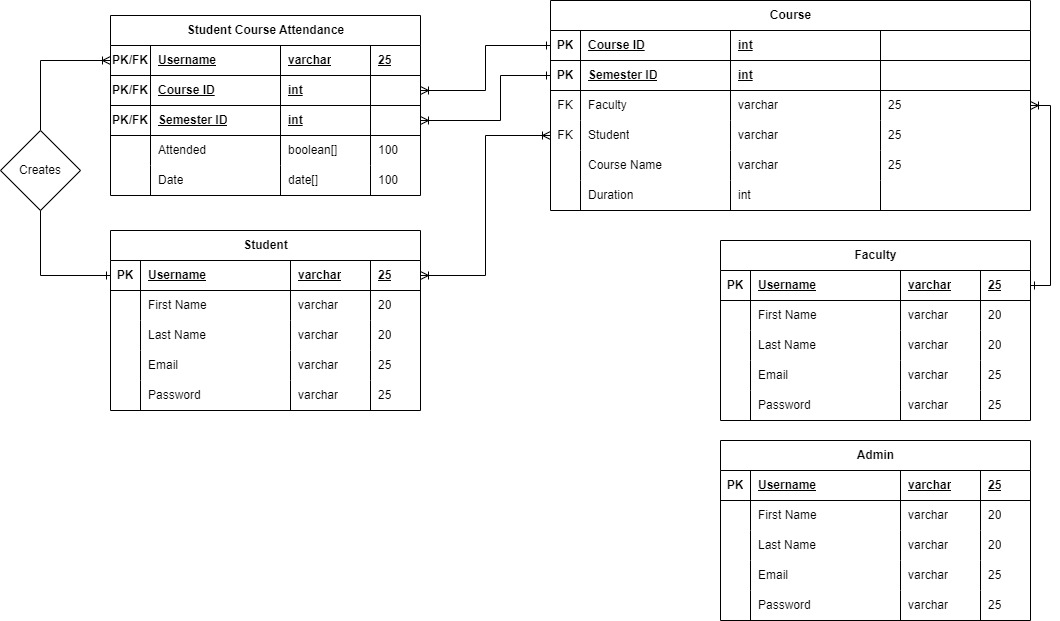
\includegraphics[scale=0.4]{Course_Model_2.jpg}
\pagebreak

\section{Data Dictionary}

\subsection{Table: Faculty}
\begin{table}[h]
    \centering
    \begin{tabular}{|l|c|c|c|c|l|}
        \hline
        \textbf{Attribute} & \textbf{Type} & \textbf{Length} & \textbf{PK/FK} & \textbf{Null?} & \textbf{Description}
        \\
        \hline
         Username & varchar & 255 & Y/N & No & A unique username made for every \\ &&&&& faculty member.
        \\
        \hline
        First Name & varchar & 255 & N/N & No & Faculty members first name.
        \\
        \hline
        Last Name & varchar & 255 & N/N & No & Faculty members last name.
        \\
        \hline
        Email & varchar & 255 & N/N & No & An email address assigned to each \\ &&&&& faculty member.
        \\
        \hline
        Password & varchar & 255 & N/N & No & A password every faculty member \\ &&&&& makes. 
        \\
        \hline
    \end{tabular}
\end{table}

The faculty table is in Third Normal Form (3NF). The functional dependencies are the following:
\begin{itemize}
  \item Username - All attributes
  \item Email - All attributes
\end{itemize}
There are no other FDs in the table.

\subsection{Table: Admin}
\begin{table}[h]
    \centering
    \begin{tabular}{|l|c|c|c|c|l|}
        \hline
        \textbf{Attribute} & \textbf{Type} & \textbf{Length} & \textbf{PK/FK} & \textbf{Null?} & \textbf{Description}
        \\
        \hline
         Username & varchar & 255 & Y/N & No & A unique username made for every \\ &&&&& faculty member.
        \\
        \hline
        First Name & varchar & 255 & N/N & No & Faculty members first name.
        \\
        \hline
        Last Name & varchar & 255 & N/N & No & Faculty members last name.
        \\
        \hline
        Email & varchar & 255 & N/N & No & An email address assigned to each \\ &&&&& faculty member.
        \\
        \hline
        Password & varchar & 255 & N/N & No & A password every faculty member \\ &&&&& makes. 
        \\
        \hline
    \end{tabular}
\end{table}

The admin table is in Third Normal Form (3NF). The functional dependencies are the following:
\begin{itemize}
  \item Username - All attributes
  \item Email - All attributes
\end{itemize}
There are no other FDs in the table.

\subsection{Table: Student}
\begin{table}[h]
    \centering
    \begin{tabular}{|l|c|c|c|c|l|}
        \hline
        \textbf{Attribute} & \textbf{Type} & \textbf{Length} & \textbf{PK/FK} & \textbf{Null?} & \textbf{Description}
        \\
        \hline
         Username & varchar & 255 & Y/N & No & A unique identifier for each student \\ &&&&& and will be used as the primary key \\ &&&&& to uniquely identify each student in \\ &&&&& the system.
        \\
        \hline
        First Name & varchar & 255 & N/N & No & The first name of the student.
        \\
        \hline
        Last Name & varchar & 255 & N/N & No & The last name of the student.
        \\
        \hline
        Email & varchar & 255 & N/N & No & The email address of the student. 
        \\
        \hline
        Password & varchar & 255 & N/N & No & The password associated with the \\ &&&&& student's account.
        \\
        \hline
    \end{tabular}
\end{table}

The student table is in Third Normal Form (3NF). The functional dependencies are the following:
\begin{itemize}
  \item Username - All attributes
  \item Email - All attributes
\end{itemize}
There are no other FDs in the table.

\subsection{Table: Student Course Attendance}
\begin{table}[h]
    \centering
    \begin{tabular}{|l|c|c|c|c|l|}
        \hline
        \textbf{Attribute} & \textbf{Type} & \textbf{Length} & \textbf{PK/FK} & \textbf{Null?} & \textbf{Description}
        \\
        \hline
         Username & varchar & 255 & N/Y & No & Identifier for the student.
        \\
        \hline
        CourseID & integer &  & N/Y & No & Identifies the course associated \\ &&&&& with the attendance record.
        \\
        \hline
        SemesterID & integer &  & N/Y & No & Identifies the semester for the \\ &&&&& attendance record.
        \\
        \hline
        Attended & boolean & 255 & N/N & No & Indicates whether the student attended \\ &&&&& (true) or did not attend (false).
        \\
        \hline
        Date & date &  & N/N & No & The date of the class session. 
        \\
        \hline
    \end{tabular}
\end{table}

The student course attendance table is in Third Normal Form (3NF). The functional dependencies are the following:
\begin{itemize}
  \item Username - All attributes
  \item CourseID - Attended
  \item SemesterID - Attended 
  \item Date - Attended 
\end{itemize}
There are no other FDs in the table.

\newpage
\subsection{Table: Course}
\begin{table}[h]
    \centering
    \begin{tabular}{|l|c|c|c|c|l|}
        \hline
        \textbf{Attribute} & \textbf{Type} & \textbf{Length} & \textbf{PK/FK} & \textbf{Null?} & \textbf{Description}
        \\
        \hline
         CourseID & integer &  & Y/N & No & Unique identifier for the course.
        \\
        \hline
        SemesterID & integer &  & N/N & No & Identifies the semester in which the \\ &&&&& course is offered.
        \\
        \hline
        Faculty & varchar & 255 & N/N & No & The faculty memeber teaching the \\ &&&&& course.
        \\
        \hline
        Student & varchar & 255 & N/N & No & The student enrolled in the course. \\ &&&&& This design assumes a direct link, \\ &&&&& which is not typically in \\ &&&&& many-to-many relationships.
        \\
        \hline
        CourseName & varchar & 255 & N/N & No & The name of the course.
        \\
        \hline
    \end{tabular}
\end{table}

The course table is in Third Normal Form (3NF). The functional dependencies are the following:
\begin{itemize}
  \item CourseID - All attributes
  \item SemesterID - All attributes
  \item Faculty - All attributes
  \item Student - All attributes
  \item CourseName - All attributes
\end{itemize}
There are no other FDs in the table.

\chapter{COMPONENT DESIGN}

Each of the following describes the functionality at the component level of the software. Each component is described at a high level.

\section{Model Methods}

\subsection{School}
\begin{enumerate}
    \item \textbf{setAttributes} - The setAttributes method shall set the information about a school in the system.
\end{enumerate}

\subsection{User}
\begin{enumerate}
    \item \textbf{setUserAttributes} - The set user attributes method shall set the attributes of a user that come in as user input.
    \item \textbf{receiveTemporaryPassword} - The receiveTemporaryPassword method shall send a user an email containing their temporary password to login to the system.
    \item \textbf{setPassword} - The setPassword method shall take the received input from the user and set the password attribute accordingly.
    \item \textbf{resetPassword} - The resetPassword method shall take the received input from the user and set the password attribute accordingly.
    \item \textbf{login} - The login method shall receive the user input for username and password and log them in if the account exists with their permissions.
\end{enumerate}

\subsection{Admin}
\begin{enumerate}
    \item \textbf{createAdminAccount} - The createAdminAccount method shall allow an admin to create an account for a new admin. The admin shall have access rights to add a new admin and a registration form shall be displayed.
    \item \textbf{createFacultyAccount} - The createFacultyAccount method shall allow an admin to create a new account and set it as a faculty role.
    \item \textbf{editFacultyAccount} - The editFacultyAccount method shall allow an admin to edit a faculty account.
    \item \textbf{deleteFacultyAccount} - The deleteFacultyAccount method shall allow an admin to delete a faculty account.
    \item \textbf{createStudentAccount} - The createStudentAccount method shall allow an admin to create a new account and set it as a student role.
    \item \textbf{editStudentAccount} - The editStudentAccount method shall allow an admin to edit a student account.
    \item \textbf{deleteStudentAccount} - The deleteStudentAccount method shall allow an admin to delete a student account.
    \item \textbf{createCourse} - The createCourse method shall allow an admin to create a new course in the system.
    \item \textbf{editCourse} - The editCourse method shall allow an admin to edit a course's information.
    \item \textbf{deleteCourse} - The deleteCourse method shall allow an admin to delete a course from the system.
\end{enumerate}

\subsection{Faculty}
\begin{enumerate}
    \item \textbf{bulkOnBoard} - The bulkOnBoard method shall run on "upload" button click. It shall then check for faculty authorization to allow a faculty member to upload a csv file containing student information. It shall then store all the student information from the file.
    \item \textbf{individualOnBoard} - Might be createStudentAccount().
    \item \textbf{addStudentToCourse} - The addStudentToCourse method shall add a student to a course.
    \item \textbf{removeStudentFromCourse} - The removeStudentFromCourse shall remove a student from the selected enrolled course.
    \item \textbf{editStudentInformation} - The editStudentInformation method shall allow that a faculty member to change a student's information.
    \item \textbf{createStudentAccount} - The createStudentAccount method shall allow that a faculty member create a new student account. Faculty shall input student name and email, and the information shall be saved to the system.
    \item \textbf{deleteStudentAccount} - The deleteStudentAccount method shall allow a faculty member to completely delete a student account and related attendance records from the system.
    \item \textbf{addAttendanceRecord} - The addAttendanceRecord method shall allow a faculty member to add a new attendance record for the course.
    \item \textbf{editAttendanceRecord} - The editAttendanceRecord method shall allow a faculty member to edit any attendance record for a course.
    \item \textbf{deleteAttendanceRecord} - The deleteAttendanceRecord method shall allow a faculty member to delete any attendance record for a course.
\end{enumerate}

\subsection{Student}
\begin{enumerate}
    \item \textbf{setupAccount} - The setupAccount method shall allow a student to finish their account setup.
    \item \textbf{viewStudentInformation} - The viewStudentInformation method shall display the individual student's account information minus sensitive information.
    \item \textbf{trackAttendance} - The trackAttendance method shall allow a user to enter the attendance code displayed by a faculty member to track their attendance.
\end{enumerate}

\subsection{Course}
\begin{enumerate}
    \item \textbf{setAttributes} - The setAttributes method shall set the information about a course.
    \item \textbf{getAttributes} - The getAttributes method shall return the information about a course.
    \item \textbf{addStudent} - The addStudent method shall add a student to the course.
    \item \textbf{removeStudent} - The remove student method shall remove a student from a course.
    \item \textbf{addFaculty} - The addFaculty method shall assign a faculty member to the course and update that information in the system.
    \item \textbf{removeFaculty} - The removeFaculty method shall removed a selected faculty member from the course and update that information in the system.
\end{enumerate}

\subsection{AttendanceRecord}
\begin{enumerate}
    \item \textbf{setAttributes} - The setAttributes method shall set the information about an attendance record.
    \item \textbf{markAttendance} - The markAttendance method shall update the attendance record status for a student.
    \item \textbf{printAttendanceRecord} - The printAttendanceRecord shall display the attendance records.
\end{enumerate}

\subsection{OverallStudentAttendanceRecord}

\subsection{OverallCourseAttendanceRecord}

\subsection{Role}
\begin{enumerate}
    \item \textbf{setAttributes} - The setAttributes method shall set the information about a role from user input.
    \item \textbf{addRole} - The addRole method shall create a new role for the platform.
    \item \textbf{editRole} - The editRole method shall take user input information about a role and update it in the system.
    \item \textbf{deleteRole} - The deleteRole method shall delete selected roles from the system.
    \item \textbf{assignRole} - The assignRole method shall give the selected user account a role within the system.
\end{enumerate}

\section{View Methods}

\subsection{LoginView}
\begin{enumerate}
    \item \textbf{inputCredentials} - The inputCredentials method shall display necessary entry labels for username and password.
    \item \textbf{forgotPassword} - The forgotPassword method shall display a button with forgot password text that will redirect a user to the forgot password page.
\end{enumerate}

\subsection{ForgotPasswordView}
\begin{enumerate}
    \item \textbf{inputEmail} - The inputEmail method shall display a label and entry field for the user's email.
\end{enumerate}

\subsection{StudentDashboardView}
\begin{enumerate}
    \item \textbf{clickableCourses} - The clickableCoursesMethod shall display a dropdown of all enrolled courses for the student and shall redirect the student to the student course view.
    \item \textbf{profileSettings} - The profileSettingsButton shall display a clickable link with the text profile settings and will redirect the user to the profile settings view.
    \item \textbf{loadPhotoAndName} - The photoAndName method shall provide the means of displaying a picture for the user along with their name.
\end{enumerate}

\subsection{StudentCourseView}
\begin{enumerate}
    \item \textbf{viewAttendance} - The viewAttendance method shall provide a button with the text view attendance and shall redirect the user to the attendance records view.
    \item \textbf{recordAttendance} - The recordAttendance method shall provide a button with the text record attendance and shall redirect the user to the record attendance view.
\end{enumerate}

\subsection{AttendanceRecordView}
\begin{enumerate}
    \item \textbf{printIndividual} - The printIndividual method shall provide a widget for displaying the individual student's attendance record for the course.
    \item \textbf{printOverall} - The printOverall method shall provide a widget for displaying the overall attendance record for the course.
\end{enumerate}

\subsection{RecordAttendanceView}
\begin{enumerate}
    \item \textbf{displayAttendanceCode} - The displayAttendanceCode method shall create a widget that displays the attendance code.
    \item \textbf{recordAttendance} - The recordAttendance method shall create an entry widget with text prompting the user to input the attendance code. It shall also create a button with the text submit that will update the attendance record in the system.
\end{enumerate}

\subsection{FacultyDashBoardView}
\begin{enumerate}
    \item \textbf{clickableCourses} - The clickableCourses method shall display a checklist of all of the courses being taught by the faculty member logged in.
    \item \textbf{profileSettingsButton} - The profileSettingsButton method shall display a button with the text profile settings and will redirect the user to the profile settings view.
    \item \textbf{loadPhotoAndName} - The photoAndName method shall provide the means of displaying a picture for the user and their name.
\end{enumerate}

\subsection{FacultyCourseView}
\begin{enumerate}
    \item \textbf{attendanceManagementOption} - The attendanceManagementOption shall provide a link with the text attendance management that will redirect the user to the attendance management view.
    \item \textbf{courseManagementOption} - The courseManagementOption shall provice a link with the text course management that shall redirect the user to the course management view.
\end{enumerate}

\subsection{AttendanceManagementView}
\begin{enumerate}
    \item \textbf{listCourses} - The listCourses method shall provide a widget for displaying the course information.
    \item \textbf{displayRecords} - The displayRecords method shall create a button with the text display records that will redirect the user to the display records view.
    \item \textbf{addRecord} - The addRecord method shall create a button with the text add record that shall redirect the user to the add record view.
    \item \textbf{editDeleteRecord} - The editDeleteRecord shall create a button with the text edit/delete record that shall redirect the user to the edit/delete record view.
    \item \textbf{printReport} - The printReport method shall create a widget that shall display the course's attendance report.
\end{enumerate}

\subsection{DisplayRecordsView}
\begin{enumerate}
    \item \textbf{listStudentRecords} - The listStudentRecords method shall provide a widget that shall display the course's student attendance records.
    \item \textbf{printIndividualRecord} - The printIndividualRecord shall provide a widget that shall display the attendance for an individual student.
\end{enumerate}

\subsection{AddRecordView}
\begin{enumerate}
    \item \textbf{addStudentRecord} - The addStudentRecord method shall provide an input box for adding a student and relative record information. It shall also create a button for submitting the information in the system.
\end{enumerate}

\subsection{EditDeleteRecordView}
\begin{enumerate}
    \item \textbf{listStudentRecord} - The listStudentRecord method shall provide a widget for displaying all course student's records along with checkboxes.
    \item \textbf{editRecord} - The editRecord method shall provide entry widget for changing the attendance record and a button to submit.
    \item \textbf{deleteRecord} - The deleteRecord shall provide a button that deletes checked attendance records.
\end{enumerate}

\subsection{CourseManagementView}
\begin{enumerate}
    \item \textbf{listCourses} - The listCourses method shall provide a widget for displaying the list of courses to select from.
    \item \textbf{viewStudentList} - The viewStudentList method shall provide a link with the text view student list that shall redirect the user to the student list view.
    \item \textbf{modifyStudents} - The modifyStudents method shall provide a link with the text modify students that shall redirect the user to the modify students view.
    \item \textbf{bulkOnBoardStudents} - The bulkOnBoardStudents method shall provide a link with the text bulk on-board that shall redirect the user to the bulk on-board view.
\end{enumerate}

\subsection{StudentListView}
\begin{enumerate}
    \item \textbf{listStudents} - The listStudents method shall create a widget that displays the list of students with attendance.
\end{enumerate}

\subsection{ModifyStudentsView} 
\begin{enumerate}
    \item \textbf{listStudents} - The listStudentsMethod shall provide a widget that displays the list of students with checkboxes.
    \item \textbf{editStudent} - The editStudent method shall provide an entry widget for changing the student information.
    \item \textbf{deleteStudent} - The deleteStudent method shall provide a button that deletes checked students from the course. 
\end{enumerate}

\subsection{BulkOnBoardView}
\begin{enumerate}
    \item \textbf{formatGuidelines} - The formatGuidelines method shall provide a text widget that will specify the format guidelines for the file expectation.
    \item \textbf{selectFile} - The selectFile method shall provide a button that shall allow a user to select the file to upload.
    \item \textbf{displayFile} - The displayFile method shall provide a text widget that displays to the user the file uploaded.
    \item \textbf{submitFile} - The submitFile method shall provide a button with the text submit that will bulk on board the students from the csv file.
\end{enumerate}

\subsection{AdminDashboardView}
\begin{enumerate}
    \item \textbf{manageAccountsDashboard} - The manageAccountsDashboard method shall display a clickable link that will redirect the admin to the manage accounts view.
    \item \textbf{manageCoursesDashboard} - The manageCoursesDashboard method shall display a clickable link that will redirect the admin to the manage courses view.
\end{enumerate}

\subsection{ManageCoursesView}
\begin{enumerate}
    \item \textbf{listCourses} - The listCourses method shall display a table selection of all courses
    \item \textbf{viewStudents} - The viewStudents method shall display a button with the text view students that will redirect the user to the view students view.
    \item \textbf{assignFaculty} - The assignFaculty method shall display a button with the text assign faculty that shall redirect the user to the assign faculty view.
    \item \textbf{deleteCourse} - The deleteCourse method shall display a button with the text delete course that will permanently delete the course.
\end{enumerate}

\subsection{ViewStudentsView}
\begin{enumerate}
    \item \textbf{viewStudents} - The viewStudents method shall provide a widget to view all students in the course.
\end{enumerate}

\subsection{AssignFacultyView}
\begin{enumerate}
    \item \textbf{assignFaculty} - The assignFaculty method shall provide a drop down list to assign a faculty member to a specific course.
\end{enumerate}

\subsection{ManageAcountsView}
\begin{enumerate}
    \item \textbf{listUsers} - The listUsers method shall display a table selection of all users that have an account in the system.
    \item \textbf{addStudent} - The addStudent method shall display a button with the text add student that will redirect the user to the add student view.
    \item \textbf{addFaculty} - The addFaculty method shall display a button with the text add faculty that will redirect the user to the add faculty view.
    \item \textbf{editUser} - The editUser method shall display a button with the text edit user that shall redirect the user the editUser view.
    \item \textbf{deleteUser} - The deleteUser method shall delete checked users. It will provide text prompt for confirm delete.
\end{enumerate}

\subsection{AddStudentView}
\begin{enumerate}
    \item \textbf{addStudentEntry} - The addStudentEntry shall provide text boxes for input for student information and a button to confirm add the student to the system.
\end{enumerate}

\subsection{AddFacultyView}
\begin{enumerate}
    \item \textbf{addFacultyEntry} - The addFacultyEntry shall provide text boxes and input for faculty information and a button to confirm add the faculty to the system.
\end{enumerate}

\subsection{ProfileSettingsView}
\begin{enumerate}
    \item \textbf{viewProfileInformation} - The viewProfileInformation method shall display text widgets that will contain the user's nonsensitive information.
    \item \textbf{editProfileInformation} - The editProfileInformation method shall display text in an entry widget such that it can be changed and updated. It shall also have button to confirm the changes made.
\end{enumerate}

\chapter{HUMAN INTERFACE DESIGN}

\section{Overview of User Interface}

ClassMate provides multiple features for many different users. Each user will first encounter a login page. At this page, they will be able to enter their login credentials and press a login button to fully enter the system. There will also be a "Forgot Password" button in which they will then be directed to a page to enter their email address and an email will be sent to them containing information on accessing their account. Since there are multiple users for ClassMate, after a successful login, the user will be directed to either the Student Dashboard, the Teacher Dashboard, or the Administrator Dashboard depending on the credentials used. Each dashboard will have a profile settings button that will direct the user to another page when clicked and allows them to view all of their information and edit it if needed. 

From a Student user perspective, once they enter their dashboard, they will be presented with their name and a photo ID, a list of the courses they are enrolled in/have been previously enrolled in as clickable buttons, and, like previously mentioned, a button for viewing their profile settings. If the user decides to click on a course, they will be directed to another page and presented with 2 buttons: one for viewing their attendance and one for recording their attendance. When the "View Attendance" button is clicked, they will have the option to view and print an individual attendance record for a specified day or to view and print their overall attendance record which would be for the entire semester. When the "Record Attendance" button is clicked, they will be directed to a page that allows them to enter a 6-digit code, that would be provided by the teacher, and click a submit button. If the code is valid, a success message will be displayed. If the code is invalid, an error message will appear and the entry box will be cleared, allowing them to try again.

From a Teacher user perspective, once they enter their dashboard, they will be presented with their name and a photo ID, a list of the courses they teach/have taught as clickable buttons, and, like previously mentioned, a button for viewing their profile settings. If the user decides to click on a course, they will be presented with the following buttons: one for managing the course, one for managing the attendances, and one for displaying an attendance code for the day. If they choose to click the "Display Code" button, a 6-digit code will appear for students to enter on their dashboard which will record their attendance for the day. If they choose the "Attendance Management" button, they will be presented with buttons to display an attendance record, add an attendance record, edit an attendance record, delete an attendance record, or print an overall report of attendance. If they choose the "Course Management" button, they will be presented with the following buttons: one for viewing a list of the students - which will direct them to a page with a full list of students and a button to view an individual attendance report for each student; one for modifying students - which will direct them to a page with a full list of students, a button to edit information for each student, and a button to individually delete each student; and one for on-boarding students in bulk - which will direct them to a page that will give them an option to upload a CSV file of student information, an option to send a mass email out containing a registration link, an option to display the selected file, and an option to view the guidelines of how the student information file should be formatted.

From an Admin user perspective, once they enter their dashboard, they will be presented with their name and a photo ID, a button for managing accounts, a button for managing courses, and, like previously mentioned, a button for viewing their profile settings. If the user clicks the "Manage Accounts Dashboard" button, they will be directed to a page with a list of all users in the system. They will also be presented with options for adding a student, adding a teacher, editing a user, or deleting a user. For adding a student or teacher, the user will be directed to another page in which they can choose to manually input all of the information needed or they can choose to send a registration link to the student or teacher via email. If the user clicks the "Manage Courses Dashboard" button, they will be directed to a page with a list of all courses in the system. They will also be presented with options for viewing the students in a course, assigning a teacher to a course, or deleting a course.

\section{Screen Designs}

%Show mock-ups of the interface from the user's perspective. These can be hand drawn or you can use a software tool to create illustrations. Just make them as accurate as possible. Graph paper works well when hand drawing the screens.

Following are the secreen designs of class attendence software

% Including Class Attendance Software Wireframes(only Approved Wireframes) 



\begin{figure}[htbp]
  \centering
  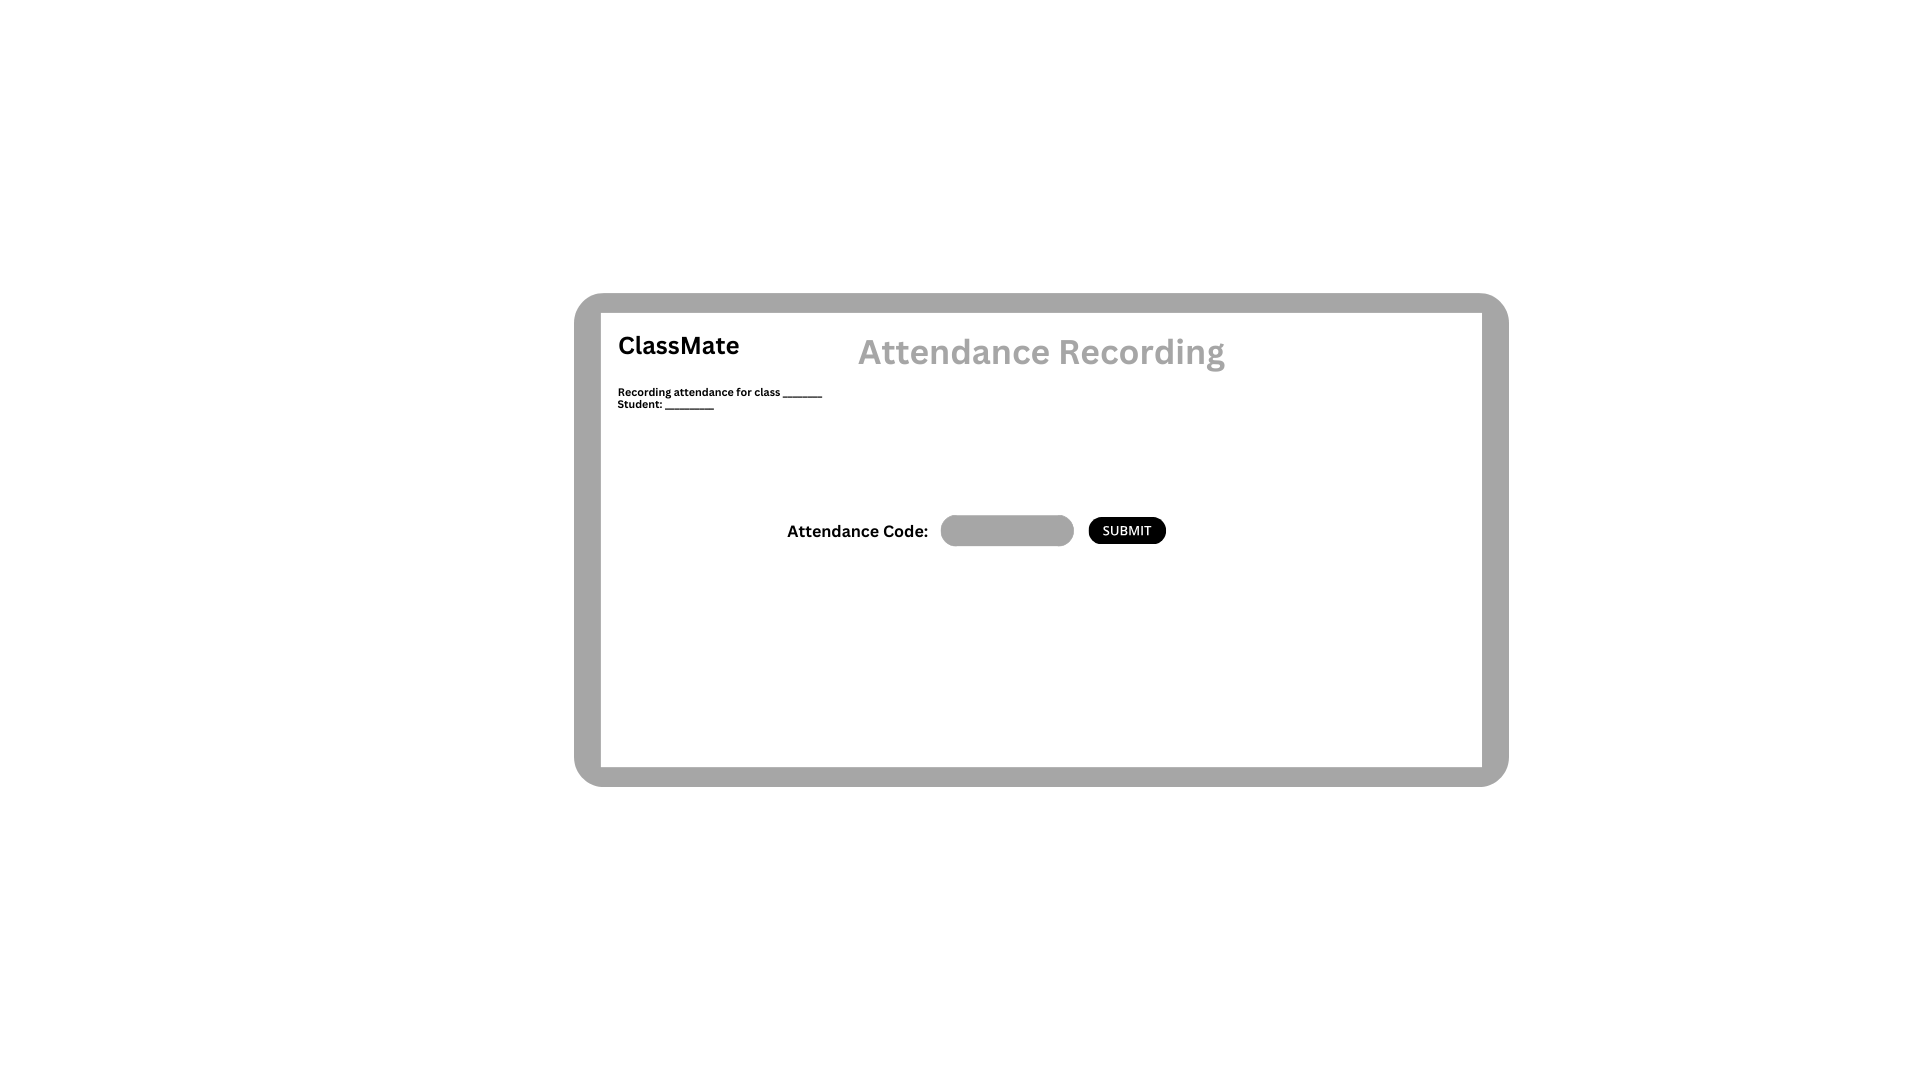
\includegraphics[width=0.5\textwidth]{Attendence_recording.png}
  \caption{Attendance Recording 1}
\end{figure}

\begin{figure}[htbp]
  \centering
  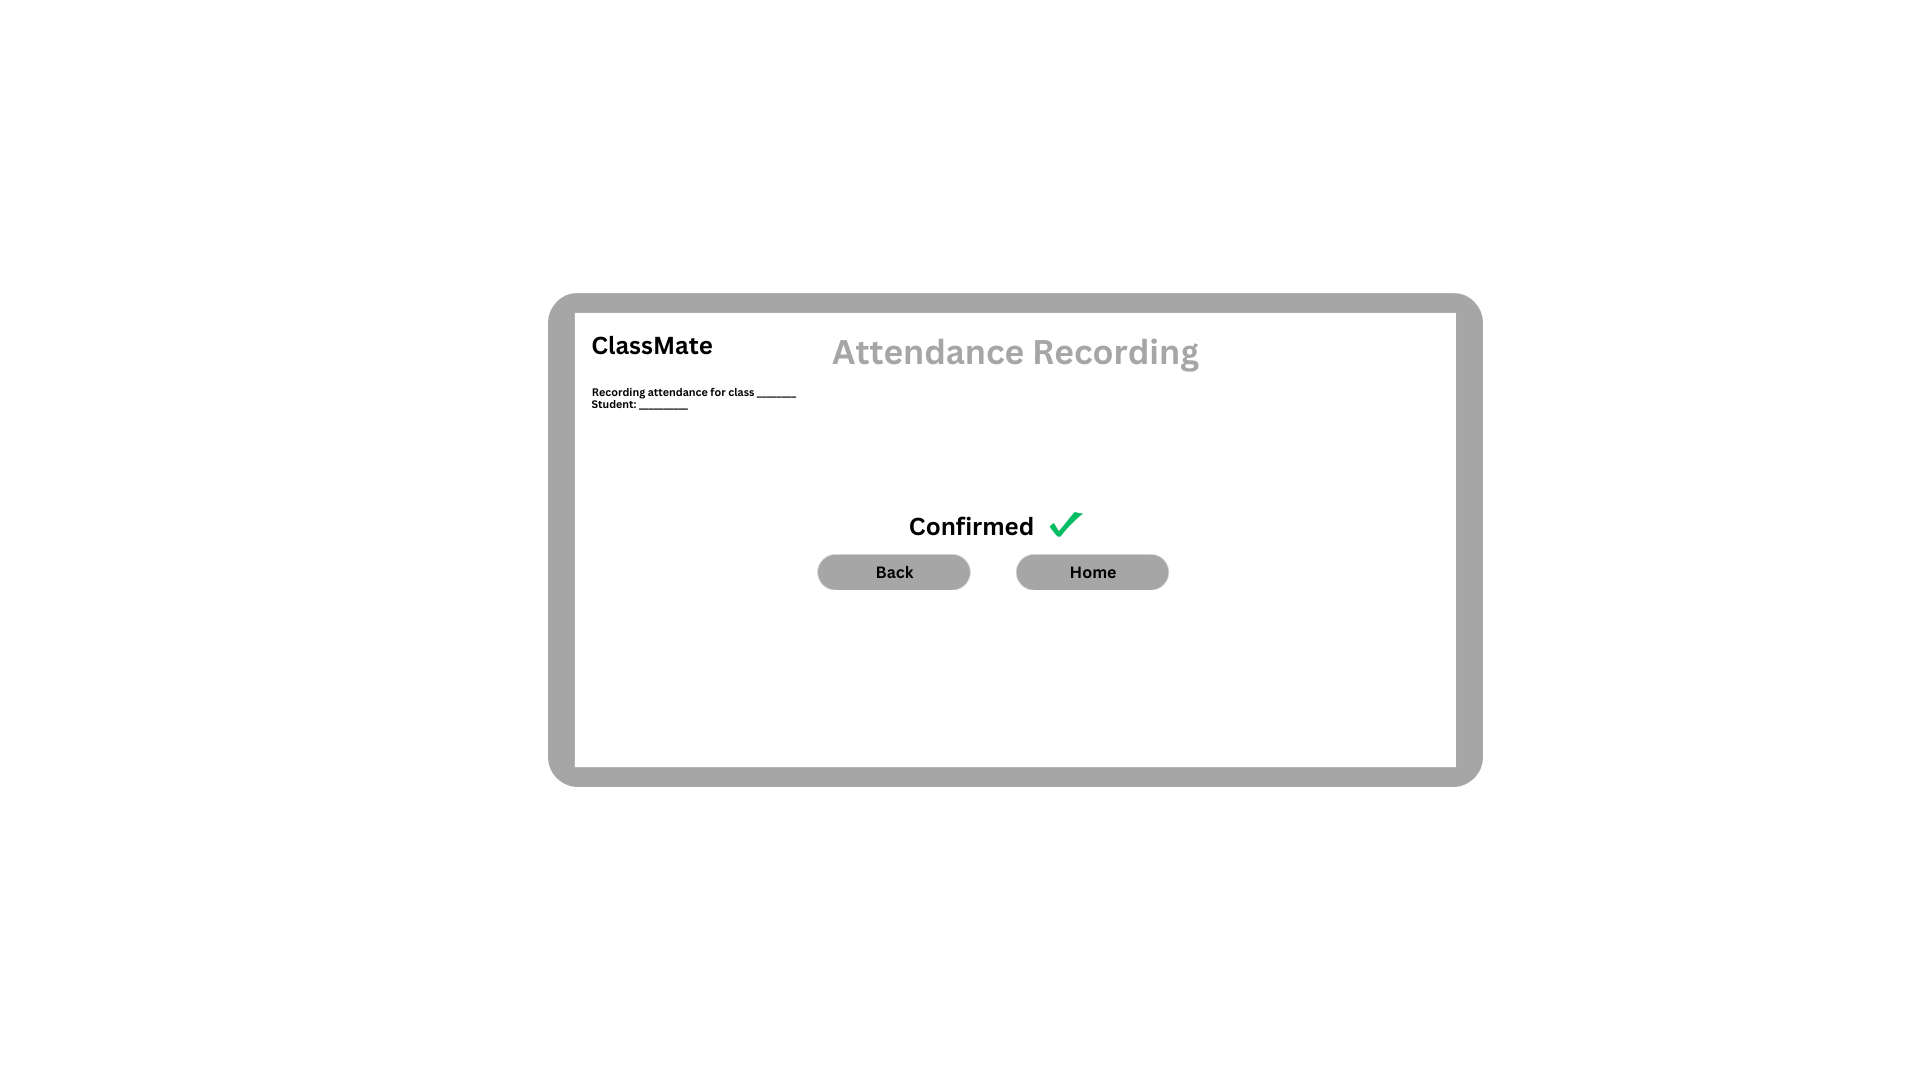
\includegraphics[width=0.5\textwidth]{Attendence_recording2.png}
  \caption{Attendance Recording 2}
\end{figure}

\begin{figure}[htbp]
  \centering
  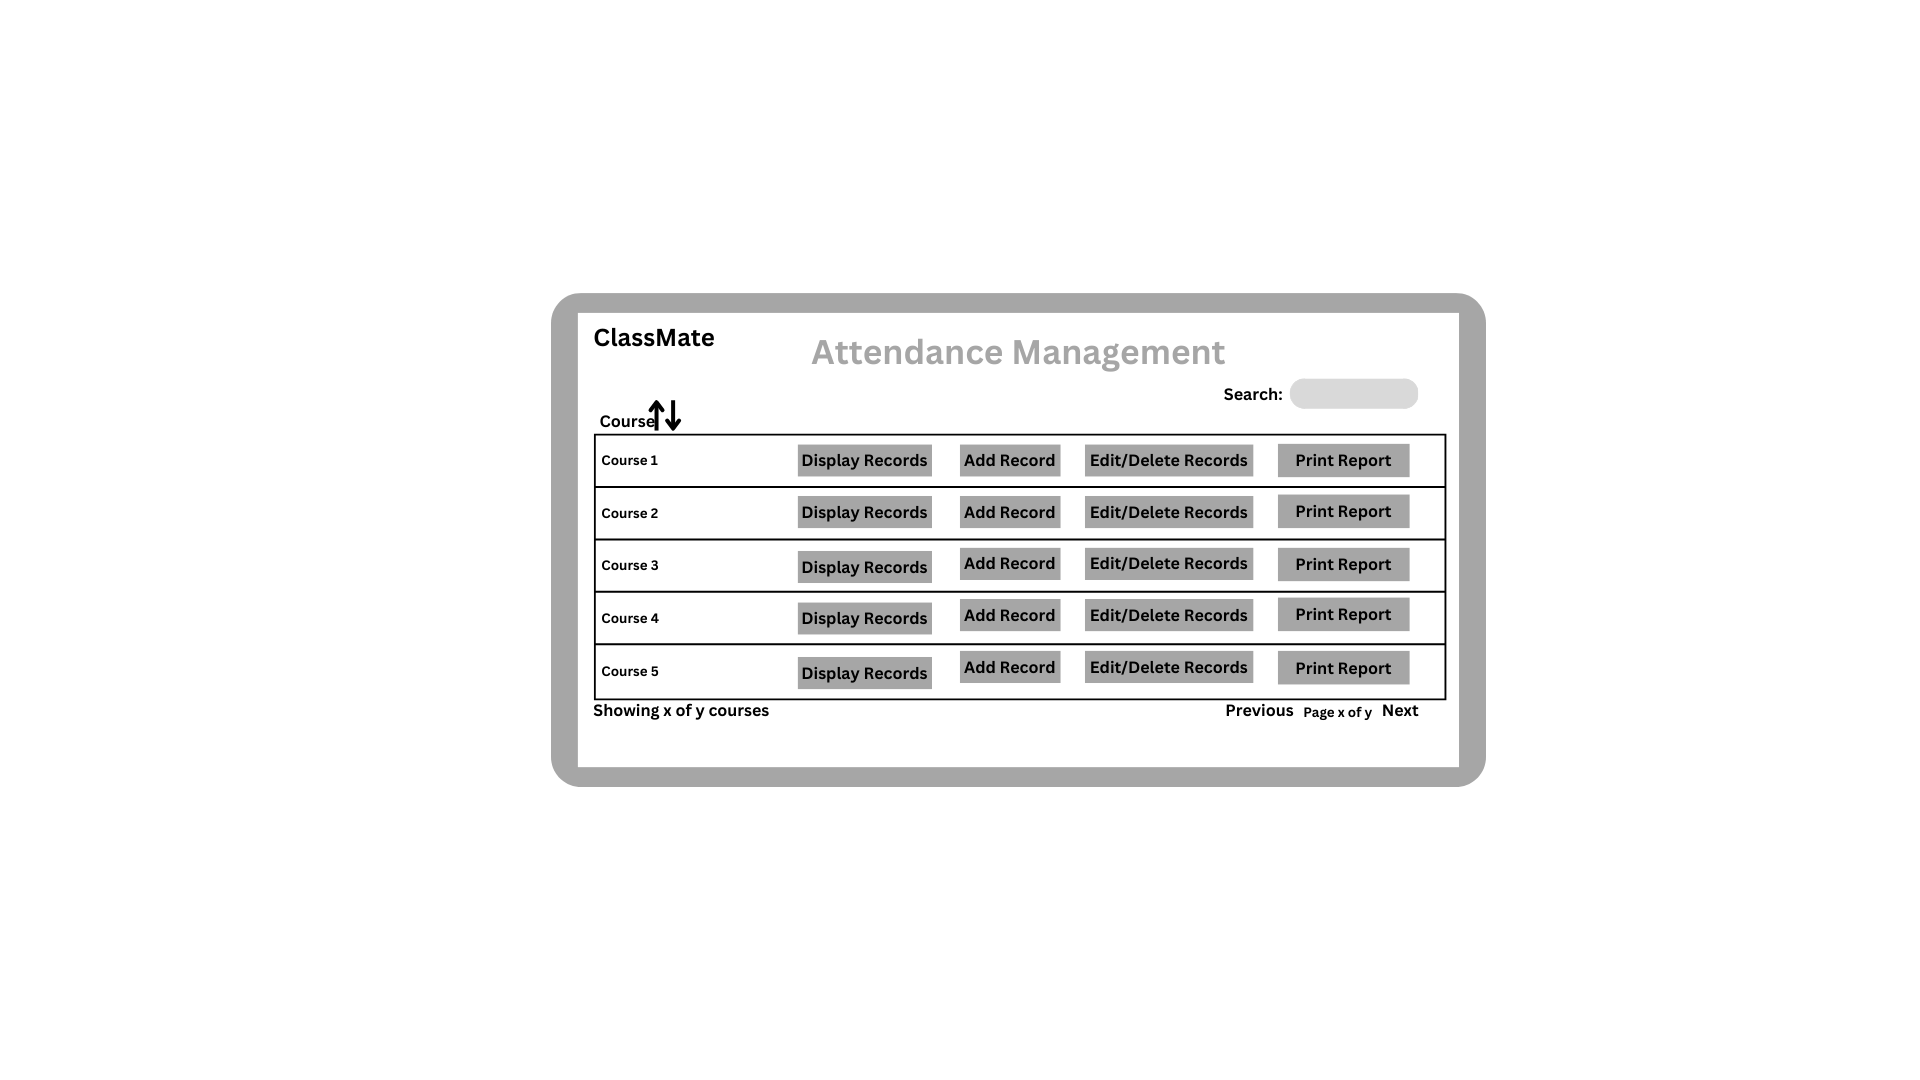
\includegraphics[width=0.5\textwidth]{Attendence_recording3.png}
  \caption{Attendance Recording 3}
\end{figure}

\begin{figure}[htbp]
  \centering
  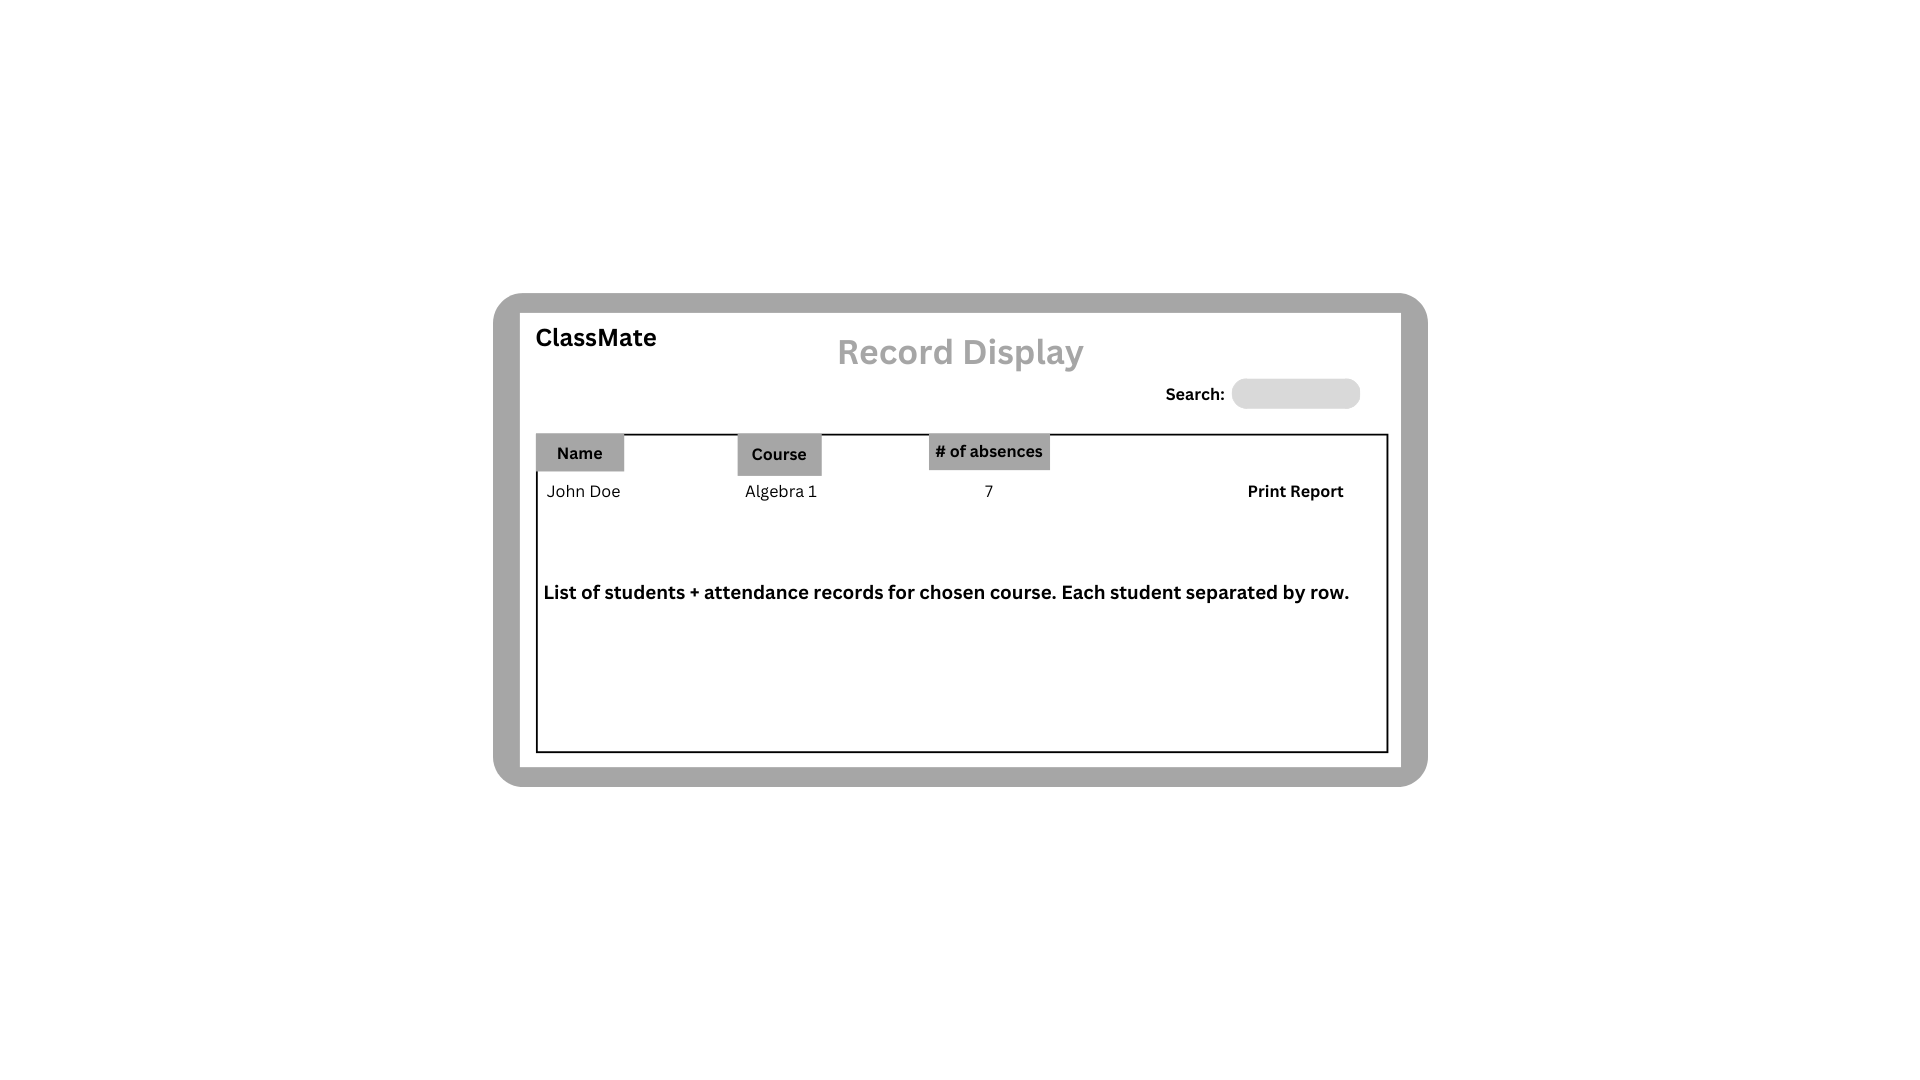
\includegraphics[width=0.5\textwidth]{Attendence_recording4.png}
  \caption{Attendance Recording 4}
\end{figure}

\begin{figure}[htbp]
  \centering
  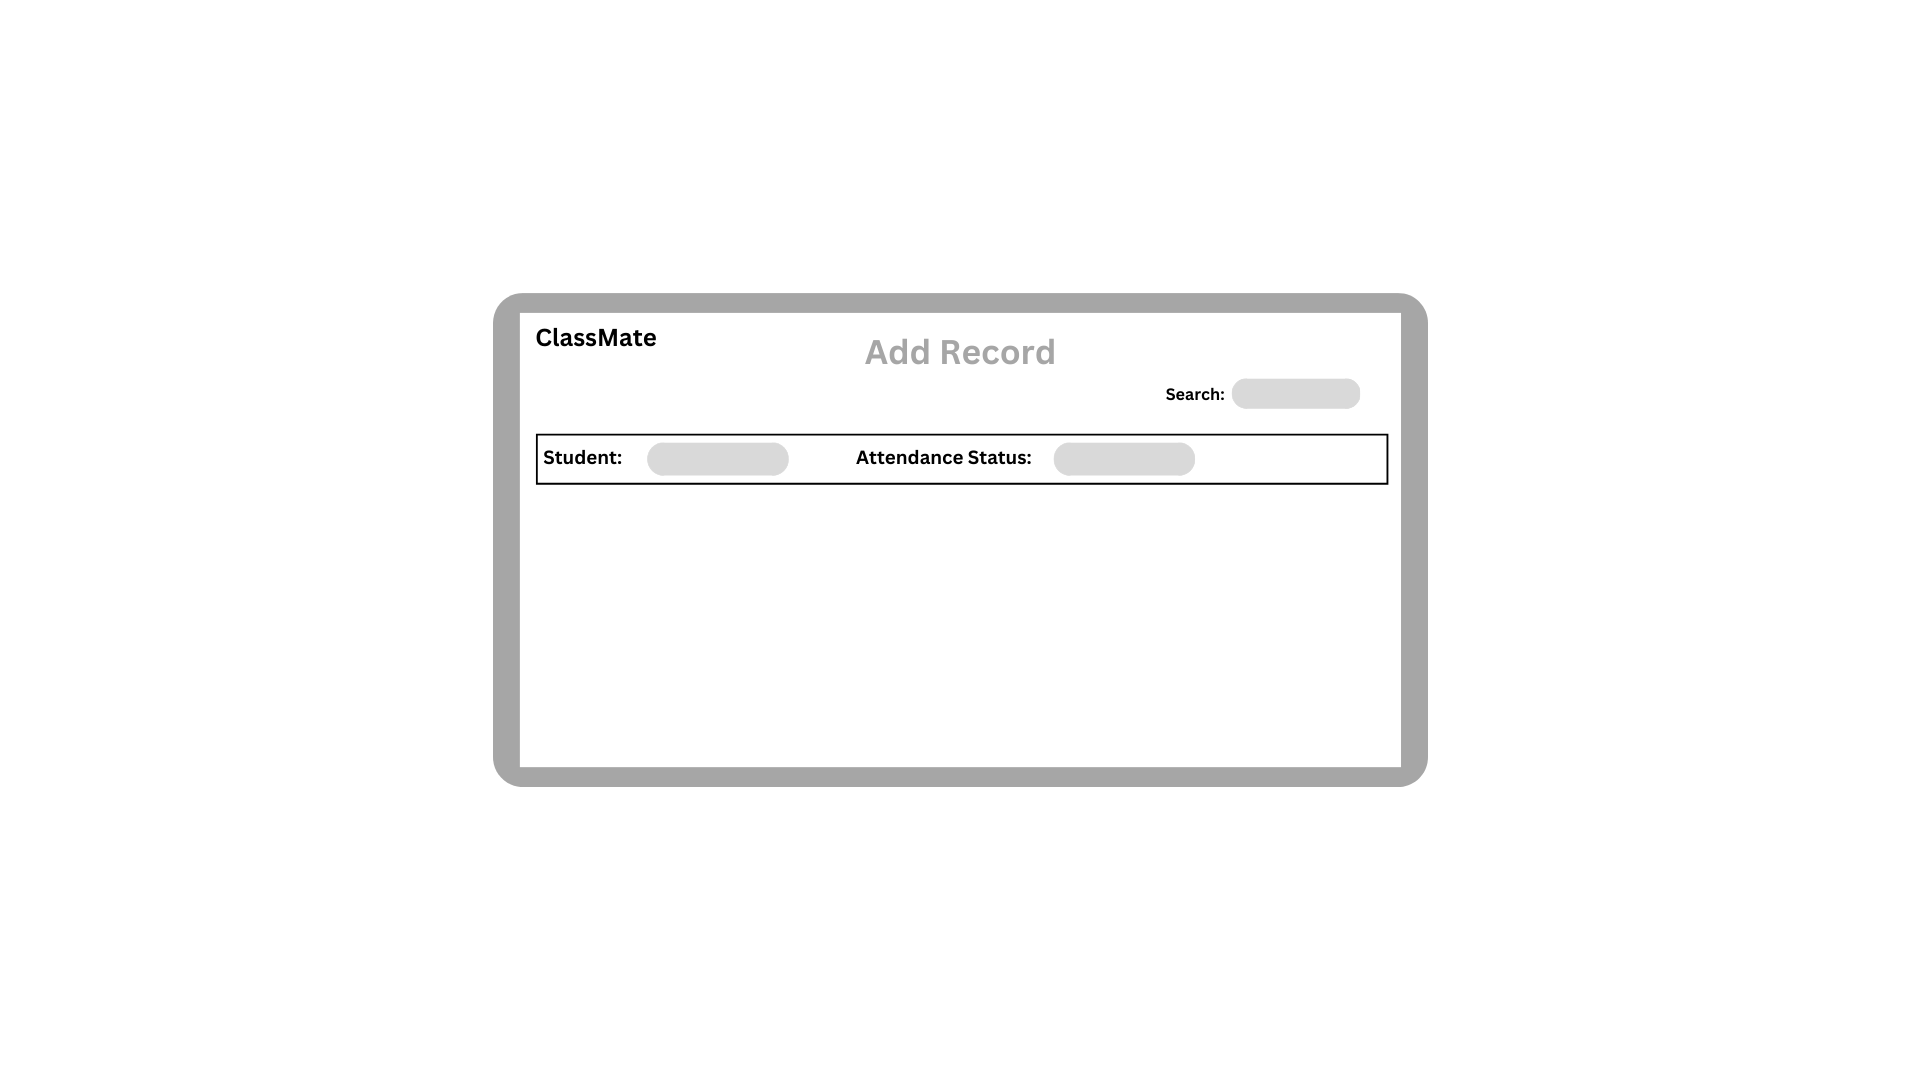
\includegraphics[width=0.5\textwidth]{Attendence_recording5.png}
  \caption{Attendance Recording 5}
\end{figure}

\begin{figure}[htbp]
  \centering
  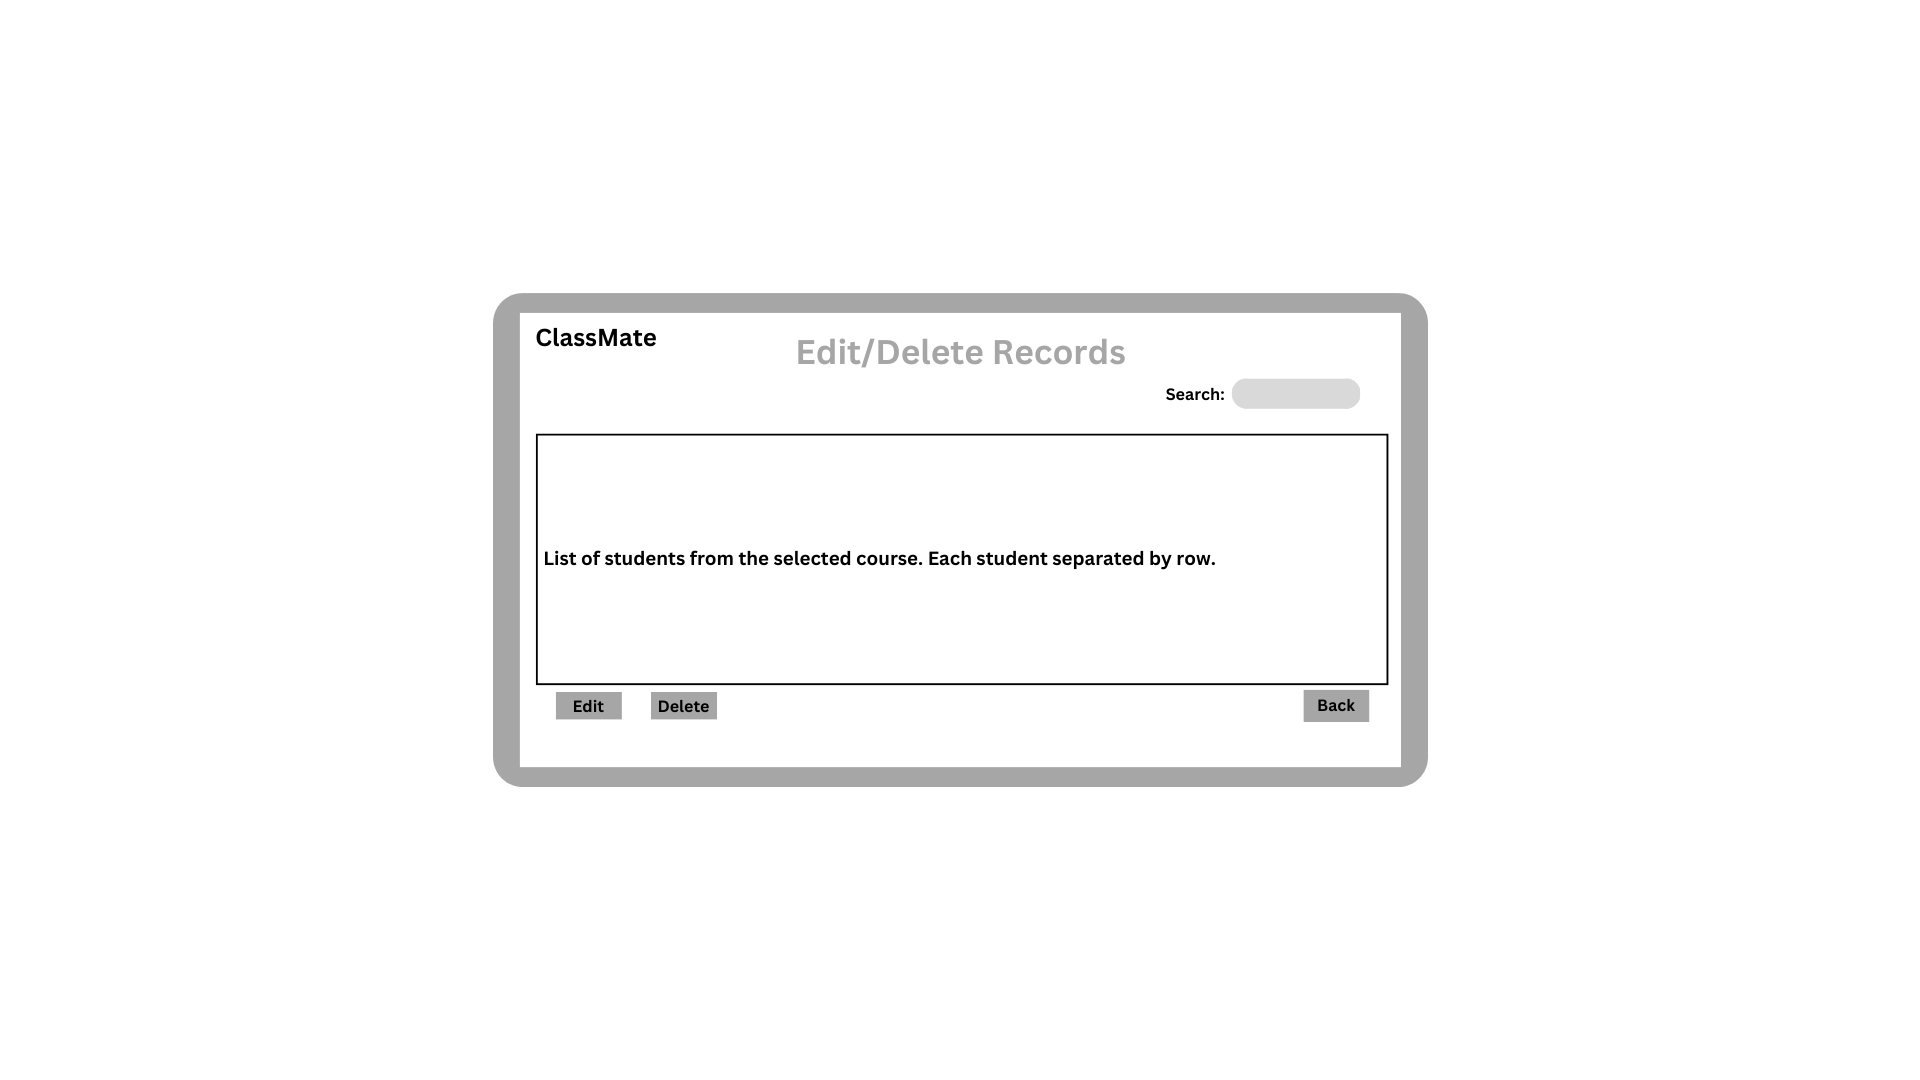
\includegraphics[width=0.5\textwidth]{Attendence_recording6.png}
  \caption{Attendance Recording 6}
\end{figure}

\begin{figure}[htbp]
  \centering
  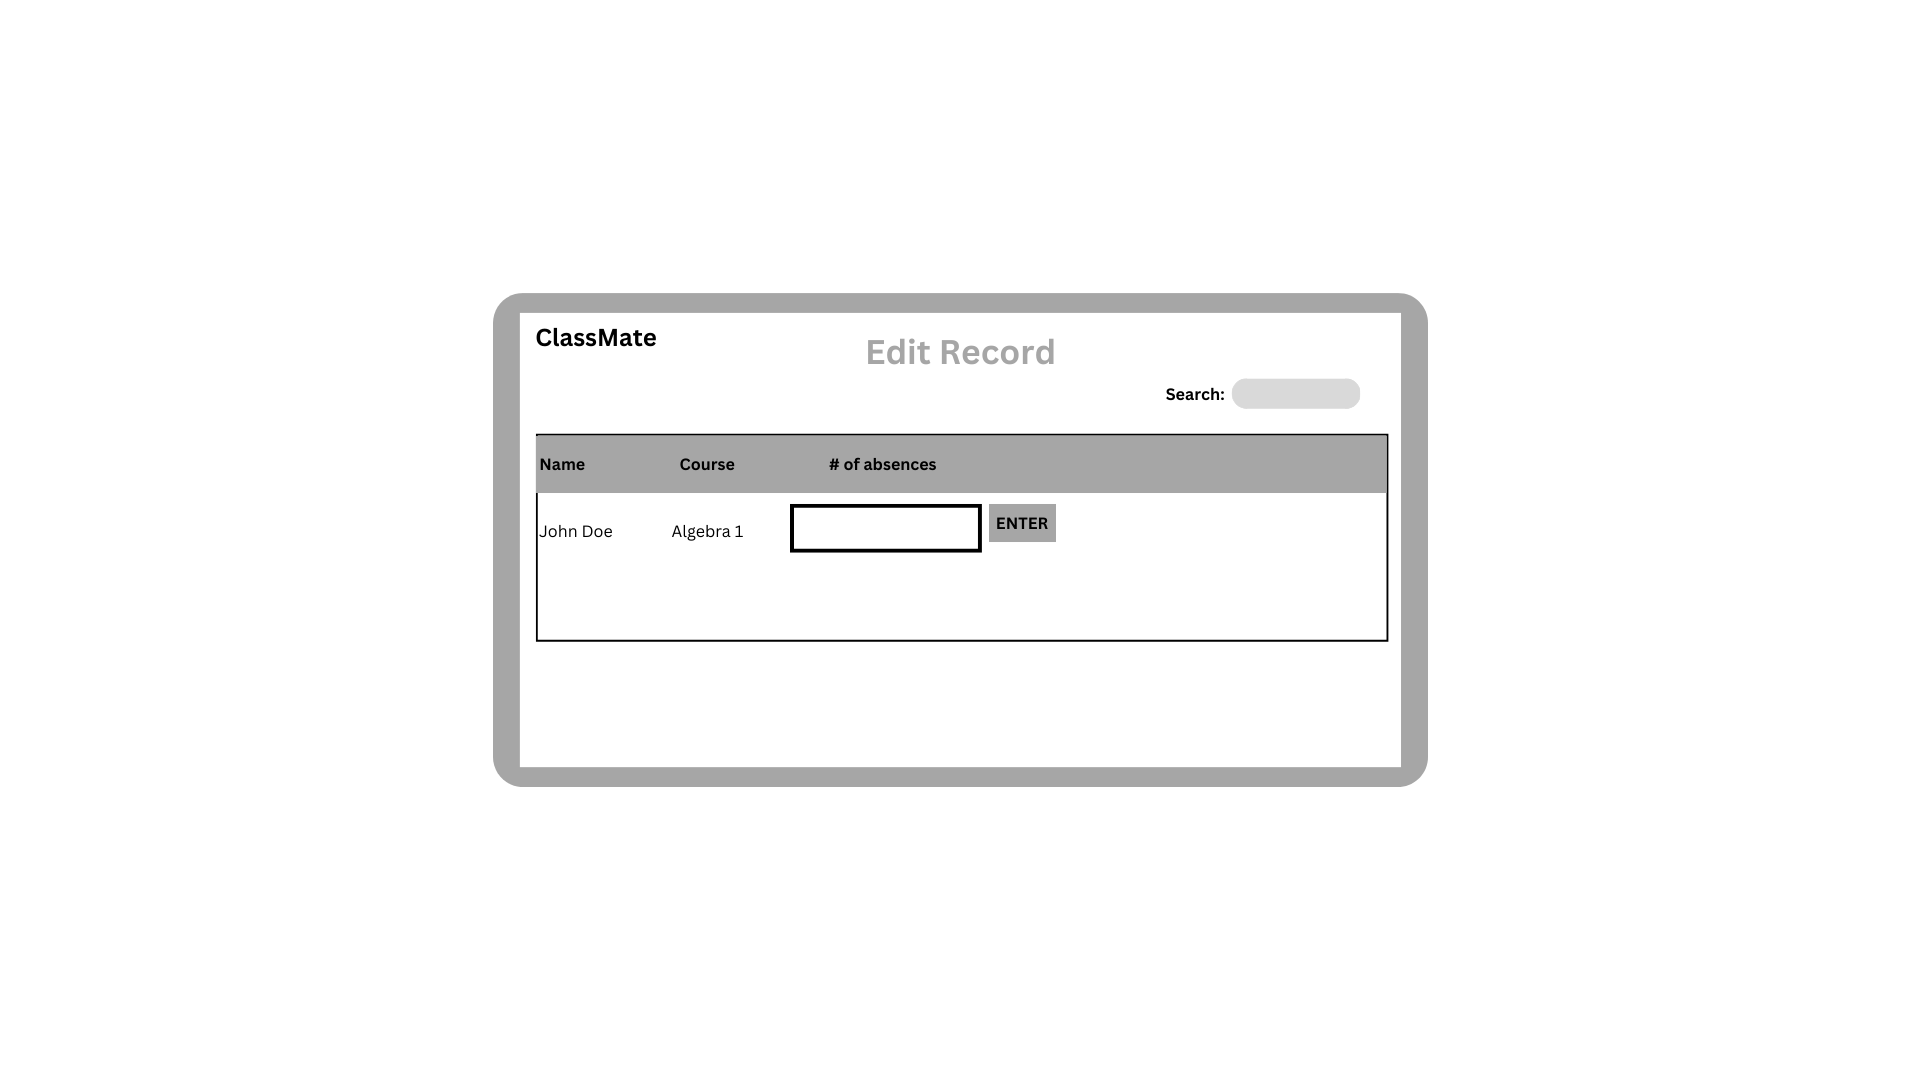
\includegraphics[width=0.5\textwidth]{Attendence_recording7.png}
  \caption{Attendance Recording 7}
\end{figure}

\begin{figure}[htbp]
  \centering
  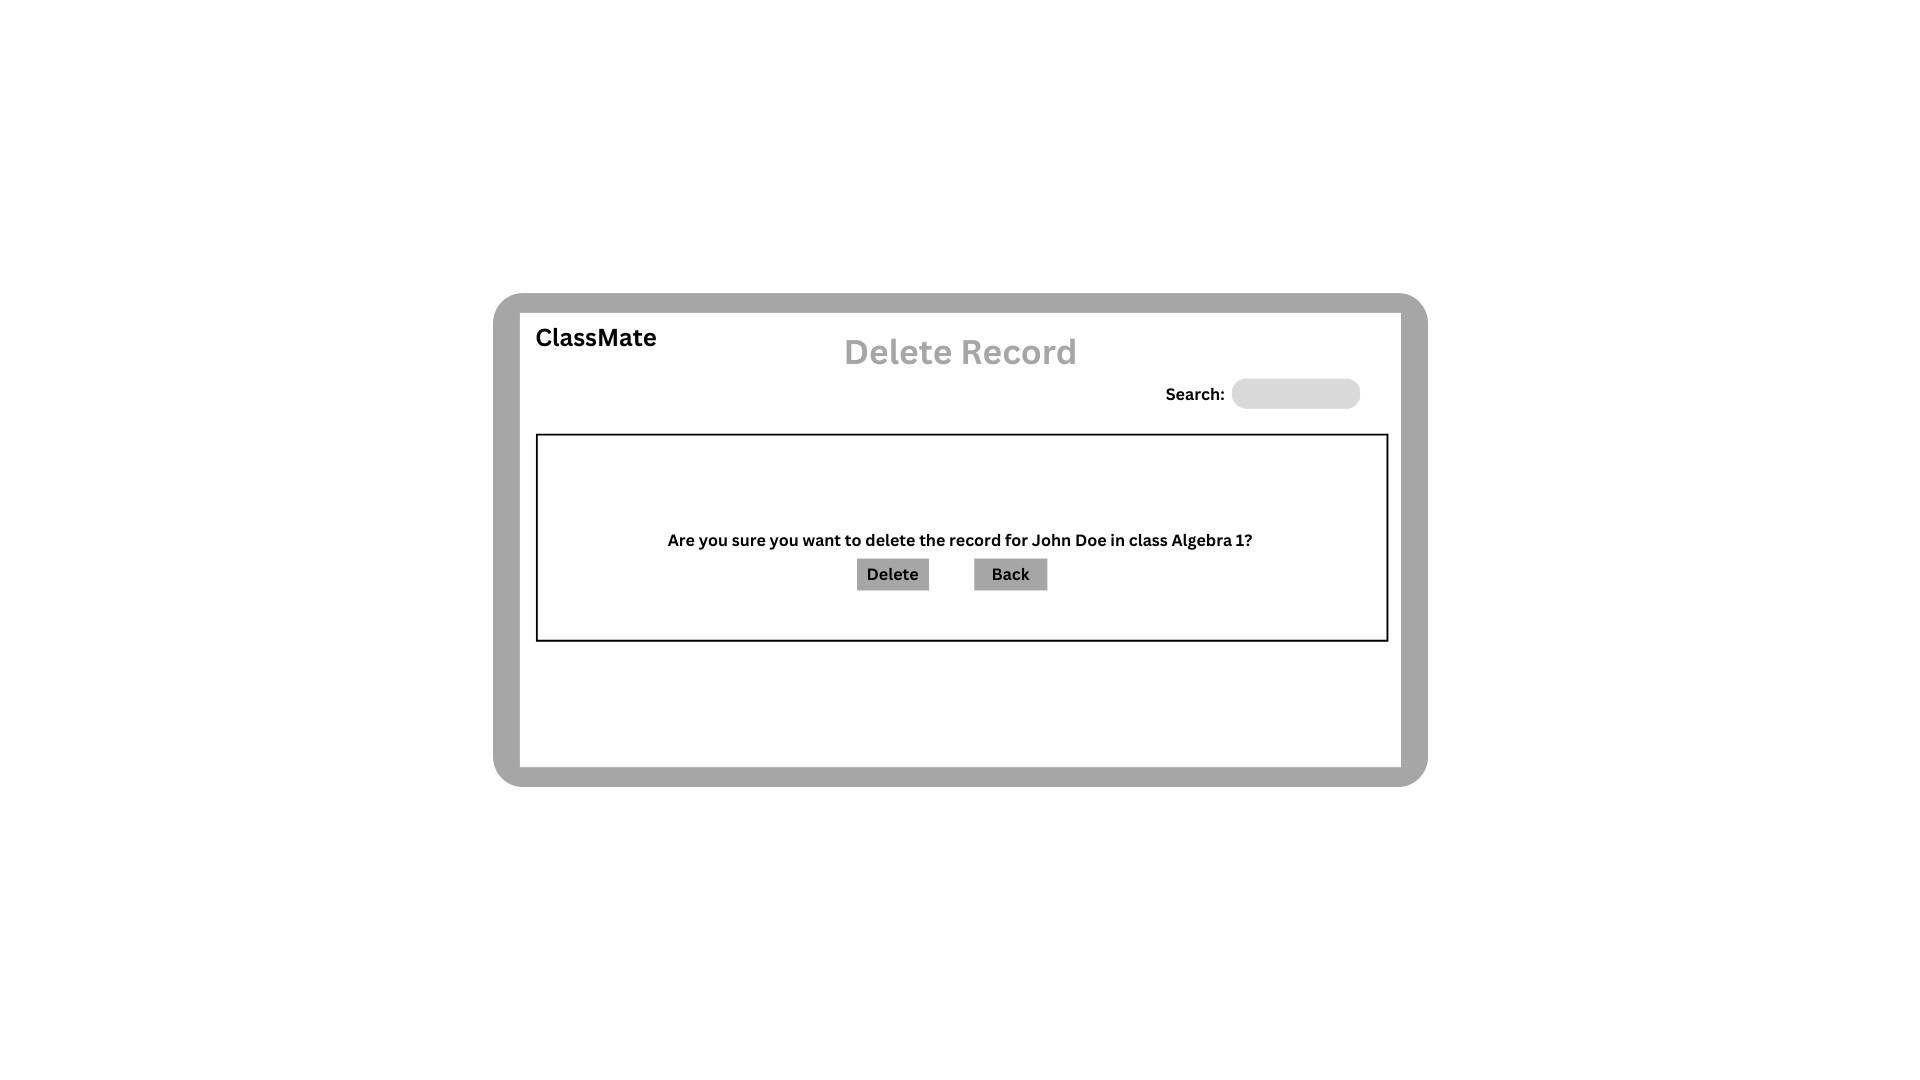
\includegraphics[width=0.5\textwidth]{Attendence_recording8.png}
  \caption{Attendance Recording 8}
\end{figure}

% Include Student Onboarding images
\begin{figure}[htbp]
  \centering
  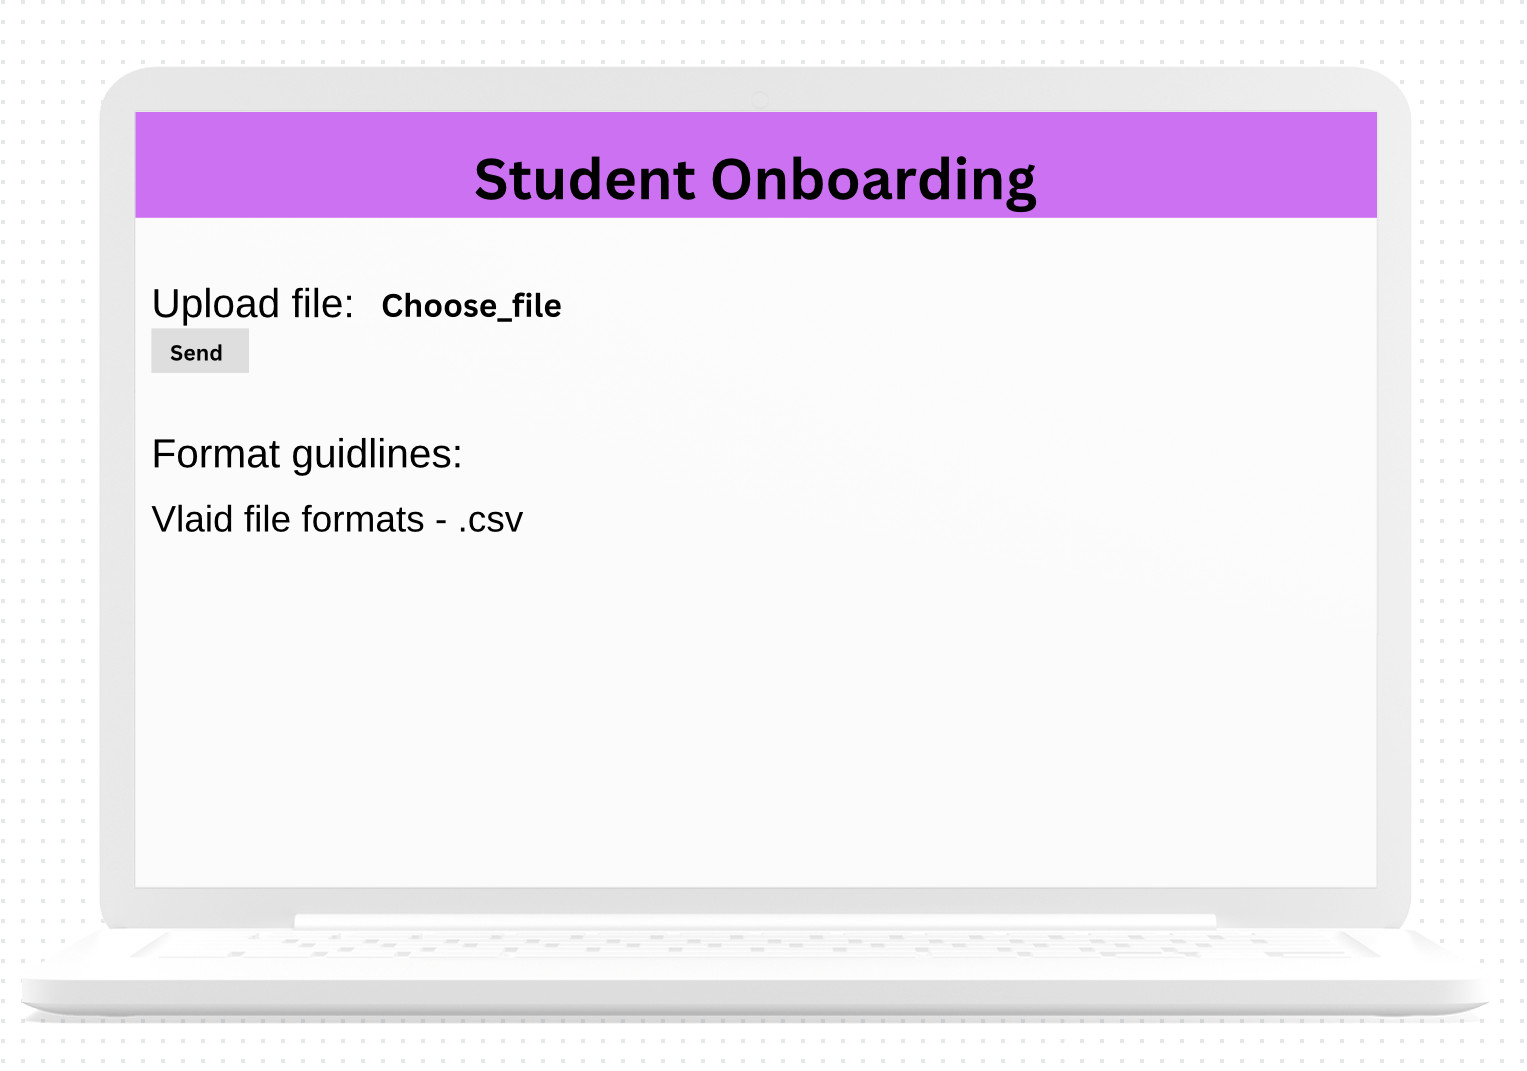
\includegraphics[width=0.5\textwidth]{Student_onboarding.png}
  \caption{Student Onboarding}
\end{figure}

\begin{figure}[htbp]
  \centering
  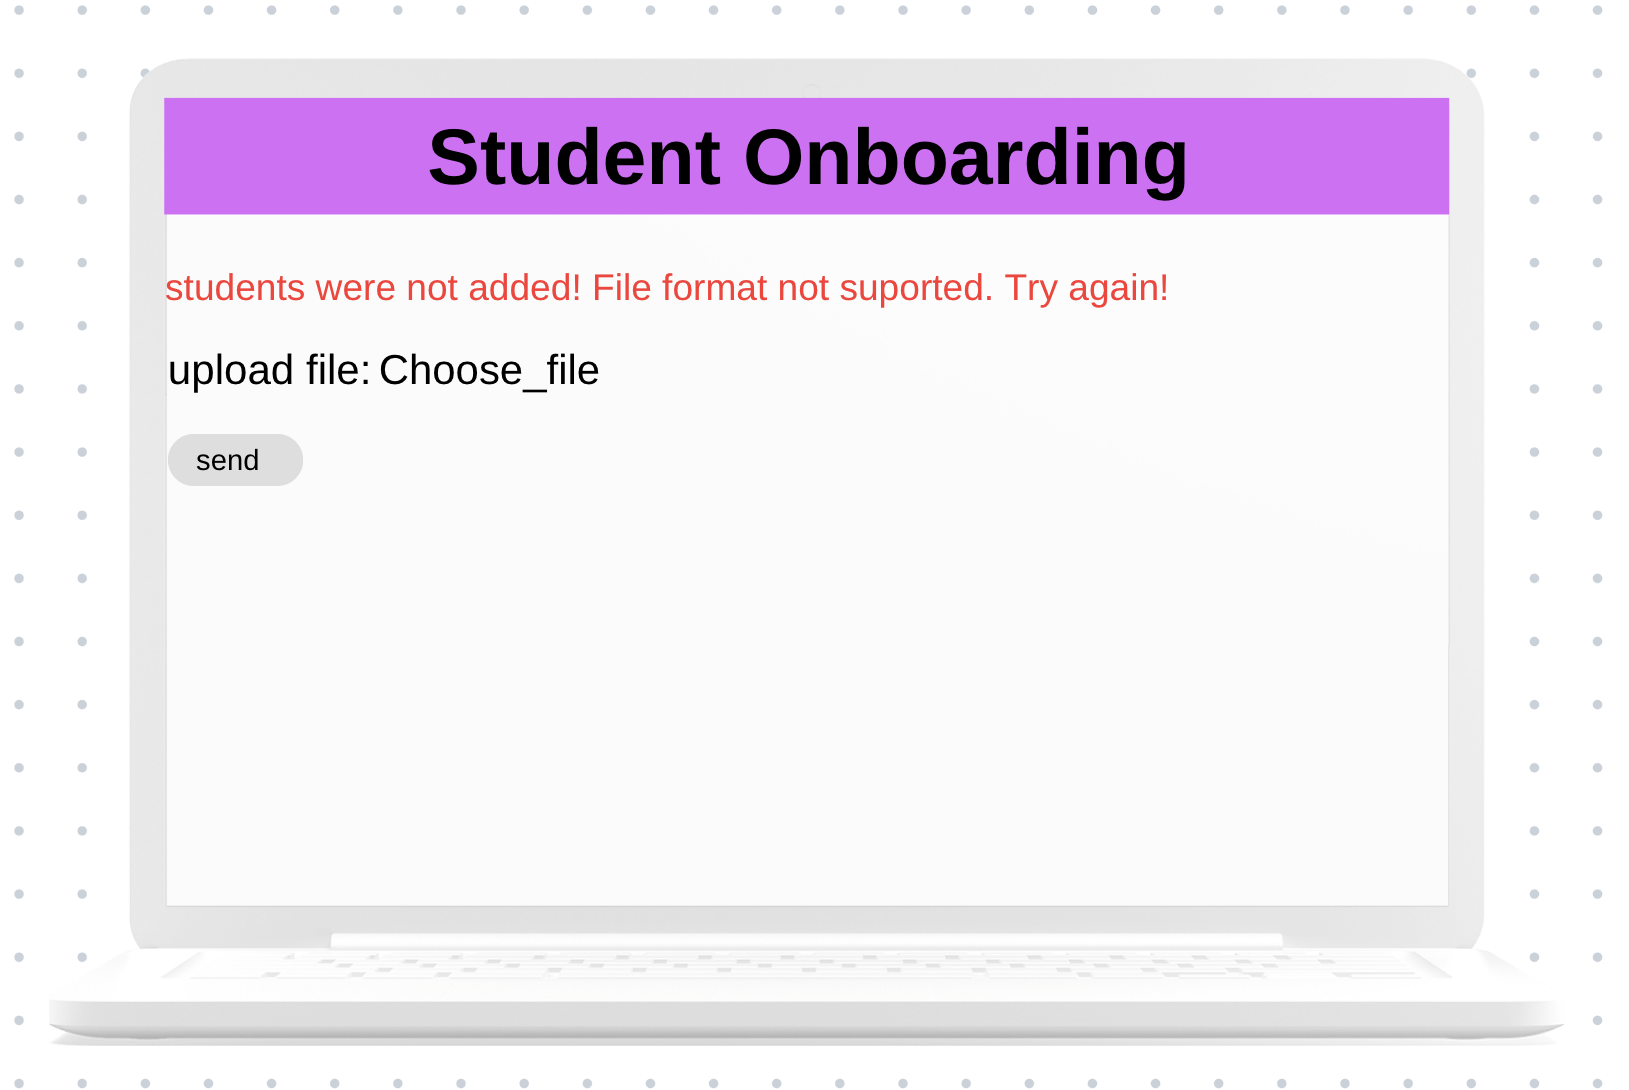
\includegraphics[width=0.5\textwidth]{Student_onboarding(InvalidFile).png}
  \caption{Student Onboarding (Invalid File)}
\end{figure}

\begin{figure}[htbp]
  \centering
  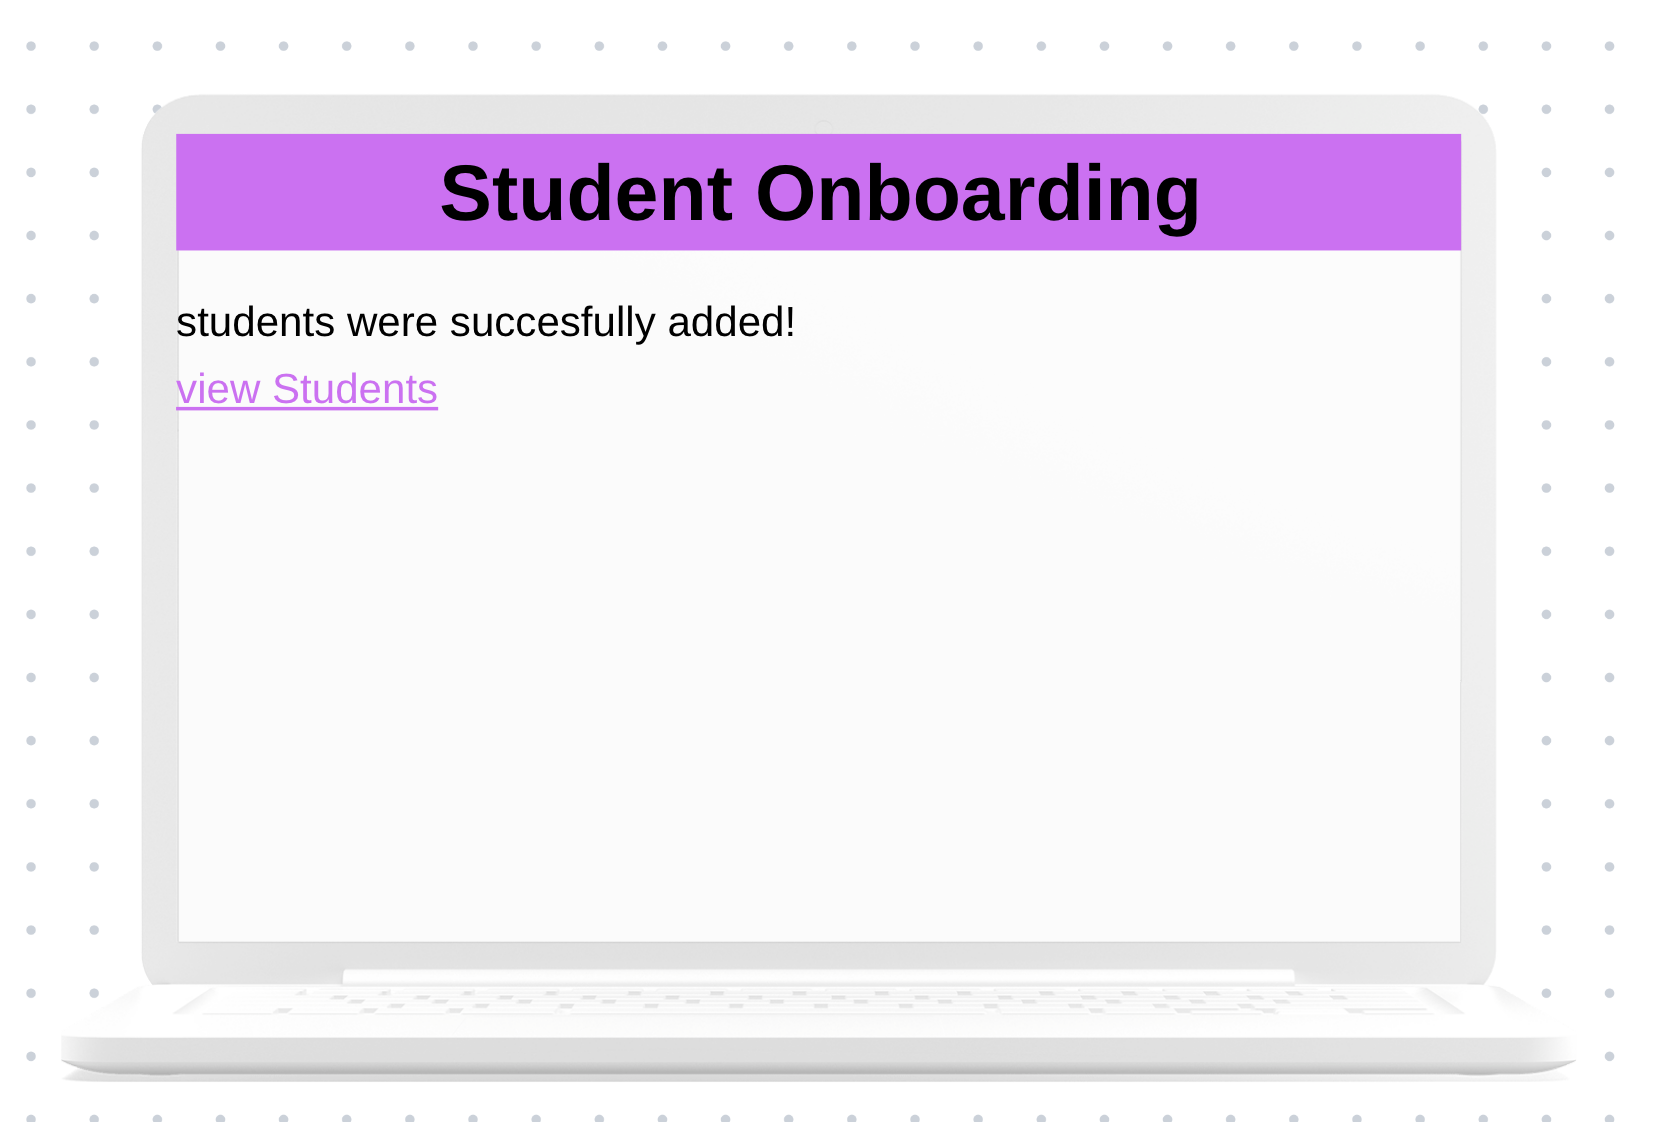
\includegraphics[width=0.5\textwidth]{Student_onboarding(succesful).png}
  \caption{Student Onboarding (Successful)}
\end{figure}



\chapter{REQUIREMENTS TRACEABILTY MATRIX}


\begin{longtable}{| p{0.6\textwidth} | p{0.60\textwidth} |}
\hline
\textbf{Requirement} & \textbf{Component/Data Structure} \\
\hline
\endhead % Header information to appear on every page
Bulk On-boarding of students by faculty & Handles bulk and individual student onboarding processes \\
\hline
Temporary Password upon Initiation for students & Manages initial login credentials and email notifications \\
\hline
Student-Centered Attendance Tracking & Tracks and records student attendance \\
\hline
Attendance Evaluation by Faculty & Generates and evaluates attendance reports \\
\hline
Classroom Management by Faculty & Manages classroom rosters and student info \\
\hline
Student Information Access & Provides access to personal and attendance information \\
\hline
Password Reset Functionality & Handles password reset processes and security checks \\
\hline
Admin Management of accounts and courses & Facilitates the creation, modification, and deletion of user accounts and courses \\
\hline
Display Attendance Code for Classes & Generates and displays attendance codes \\
\hline
Record Attendance with Code & Allows students to record attendance using a code \\
\hline
View/Print Attendance Reports (Individual/Classroom) & Generates and prints various attendance reports \\
\hline
Admin Purge of Expired Courses and Attendance Records & Manages course lifecycle and cleans up old records \\
\hline
Register Faculty and Admin Accounts & Handles the creation of faculty and admin accounts \\
\hline
Edit/Delete User Accounts and Course Information & Allows modification and deletion of user accounts and courses \\
\hline
Student Attendance Record Management (Add/Edit/Delete) & Manages detailed attendance records for students \\
\hline
Automated Email Notifications for Attendance and Account Actions & Sends automated notifications for relevant attendance and account activities \\
\hline
\end{longtable}


\end{document}